\chapter{Using the Analog Discovery 2}



This table shows the Discovery 2 to PRU-ADC cape connections.


	\begin{tabular}{llll}
%		\caption{Analog Discovery 2 Wiring}\\
		\toprule
%		\head{Wire Number} & \head{Color} & \head{PRU} & \head{BBG Header} \\
	1	& Green & Chip Select & P9 \\ 
	2	& Purple & Clock & P9 \\ 
	3	& Brown & MISO & P9 \\ 
	4	& Pink &  MOSI & P9 \\ 
	5	& Green & PRU1 Clock & P9
	\end{tabular}
	
	The repository includes a set-up file for the Analog Discovery 2 in the ``discovery2'' directory.  The Logic Analyzer will appear as in the image below.
	
	\begin{figure}[h]
		\centering
		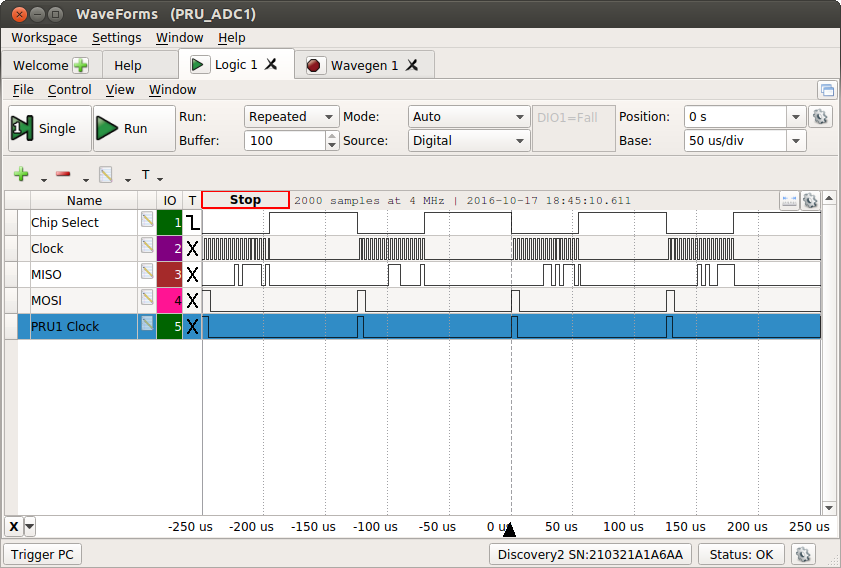
\includegraphics[width=0.9\textwidth]{photos/discovery2_logic}
		\centering\bfseries
		\caption{PRU-ADC System Diagram}
	\end{figure}
	
	The Analog Discovery also includes an audio waveform generator, and it will appear in the GUI as shown in this image:
	
		\begin{figure}[h]
			\centering
			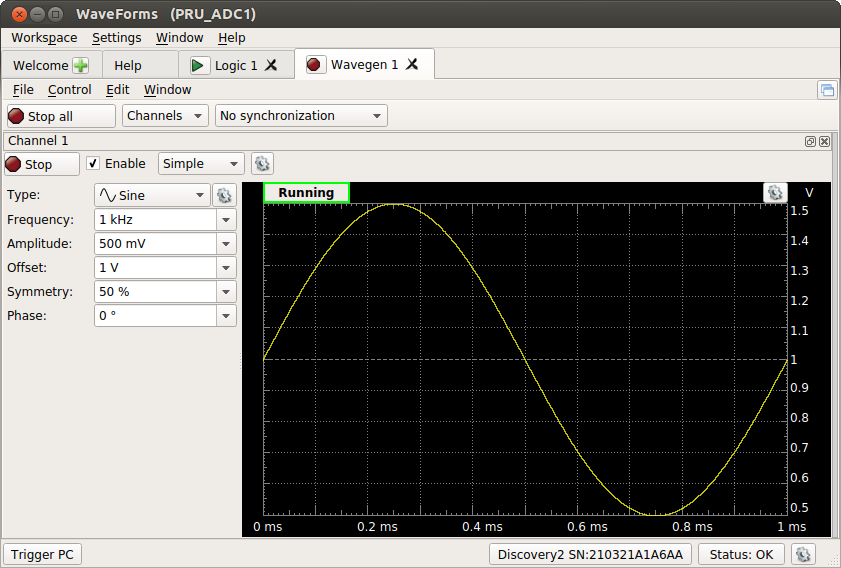
\includegraphics[width=\textwidth]{photos/discovery2_waveform}
			\centering\bfseries
			\caption{PRU-ADC System Diagram}
		\end{figure}
		


	
	
